\chapter{Background and Related Work} \label{ch:background}
	In this chapter, the concepts and definitions which are needed to implement the proposed system are identified. In the first section, the tools that are needed to build a blockchain-based strategy are introduced. In the next section, the tools and concepts borrowed from the relational database management system are identified. The last section is also dedicated to discuss the related work and the researches which have been done in this field.

		%---------------------------------- Begin of Cryptography --------------------------
		\section{Blockchain} \label{sec:blockchain}
		Blockchain technology is a distributed trusted public ledger that the stored data in it are linked using cryptography. The stored data in Blockchain are immutable and open to anyone to inspect \cite{OECD2016Science}. There are a numerous number of applications that are using Blockchain \cite{dhillon2017blockchain}, however, ‌it got its reputation because of its application as the backbone of cryptocurrencies such as Bitcoin \cite{nakamoto2008bitcoin}. 
		We utilize Blockchain technology because it is able to provide immutability and verification to the stored records in a temporal table. The immutability that the Bockchain provides makes forgeries on the records extremely difficult. Also it enables every user of the system to investigate about the trustworthiness of the records without revealing the confidential information. In this section, the ingredients of creating a Blockchain is discussed.

		\subsection{Digital signatures} \label{sec:cryptography}
			Digital signatures are the main building block of Blockchains. Blockchain utilizes digital signatures for the purpose of providing immutability and verification for its stored data. The ingredients of building a digital signatures are cryptographic keys, asymmetric encryption and hash functions that we discuss them in this section.
	%---------------------------------- End of Definition cryptography ----------------------------
	%----------------------------- Begin of Definition cryptographic keys -------------------------
			\begin{defn}[Cryptographic Keys]
				Cryptographic keys $\langle K_{priv}, K_{pub} \rangle \in \mathbf{N}^+$ are a pair of strings  that are generated using mathematical functions, where $K_{pub}$ is the public key that is accessible to everyone on the system, and $K_{priv}$ is the private key that is known only to $u$. These keys are used to encrypt/decrypt messages which are transmitted between the users\cite{stallings2017cryptography}.
			\label{dfn:cryptographic_keys}
			\end{defn}
			The procedure of creating a pair of Cryptographic keys is shown in Algorithm \ref{alg:generate_keys}.
			\begin{figure}[h]
				\begin{algorithm}[H]
					\SetAlgoLined
					\caption{Generate Cryptographic keys}
					\SetAlCapNameFnt{\tiny}
					\SetAlgoLined
					\setstretch{1.35}
					\label{alg:generate_keys}
					\DontPrintSemicolon
					 \SetKwFunction{FMain}{generateKeys}
					 \SetKwProg{Fn}{Function}{:}{}
					 \Fn{\FMain{$keySize$}}{
					    $randomVal \gets Random.new()$\;
					    $publicKey,privateKey = RSA.generate(keySize,randomVal)$ \;
					 \Return $publicKey$,$privateKey$
					}
				\end{algorithm}
			\end{figure}
	%----------------------------- End of Definition cryptographic keys -------------------------
	%----------------------------- Begin of Definition Assymetric Encryption --------------------
		
		The cryptographic keys are mainly used to encrypt data. The purppose of encryption is to convert data from their ordinary form to unintellegible information that are unreadable by unprivileged users \cite{kapoor2011cryptography}. By having a pair of cryptographic keys $\langle K_{priv}, K_{pub} \rangle$, the encryption is done asymmetrically. 

		\begin{defn}[Asymmetric Encryption]
			 Given the cryptographic keys $\langle K_{pub}, K_{priv} \rangle$ and a message $m$, an encryption technique is said to be asymmetric if:
			\begin{center}
				$c = Encrypt(K_{pub},m)$ and  $m = Decrypt(K_{priv},c)$
			\end{center}
			or
			\begin{center}
				$c = Encrypt(K_{priv},m)$ and  $m = Decrypt(K_{pub},c)$
			\end{center}
		\label{dfn:asymmetric_encryption}
		\end{defn}

		Note that, if $K_{pub}$ is known, and $E(K_{pub},m)$ is also known, in asymmetric encryption method, it is impossible to get $m$ without $K_{priv}$ \cite{stallings2017cryptography}.
		Algorithm \ref{alg:encryption} shows the basic steps to encrypt a message using $K_{pub}$ and Algorithm \ref{alg:decryption} shows the steps to decrypt a message using $K_{priv}$
		\begin{figure}[h]
			\begin{algorithm}[H]
				\caption{Encrypt a message using public key}
				\SetAlCapNameFnt{\tiny}
				\label{alg:encryption}
				\setstretch{1.35}
				\DontPrintSemicolon
				 \SetKwFunction{FMain}{encrypt}
				 \SetKwProg{Fn}{Function}{:}{}
				 \Fn{\FMain{$m$,$K_{pub}$}}{
				 	publicKeyObj = RSA.importKey($K_{pub}$)\;
				    $randomParam \gets random.choice()$\;
				 \Return publicKeyObj.encrypt($m$,$randomparam$)
				}
			\end{algorithm}
		\end{figure}


		\begin{figure}[h]
			\begin{algorithm}[H]
				\SetAlgoLined
				\caption{Decrypt an encrypted message using private key}
				\SetAlCapNameFnt{\tiny}
				\label{alg:decryption}
				\setstretch{1.35}
				\DontPrintSemicolon
				 \SetKwFunction{FMain}{decrypt}
				 \SetKwProg{Fn}{Function}{:}{}
				 \Fn{\FMain{$enc\_message$,$K_{priv}$}}{
				 	privateKeyObj = RSA.importKey($K_{priv}$)\;
				 \Return privateKeyObj.decrypt($enc\_message$)
				}
			\end{algorithm}
		\end{figure}

		In addition to asymmetric encryption, hash functions are also another ingredient of the digital signatures.
	%----------------------------- End of Definition Assymetric Encryption --------------------
	%----------------------------- Begin of Definition Hash function --------------------------
		\begin{defn}[Hash function]
			Assume $m$ to be the message with an arbitrary size chosen from domain $\mathcal{A}$. $hash(m)\rightarrow sketch$ is a function that maps the $m$ of any size from domain $\mathcal{A}$ to a fixed size string (normally 256 bits) in a smaller domain $\mathcal{B}$ \cite{aumasson2014thehash}.
		\label{dfn:hash_function}
		\end{defn}

		Now we discuss the procedure of generating a digital signature using the tools that we introduced.
	%----------------------------- End of Definition Hash function ----------------------------
	%----------------------------- Begin of Definition Digital Signature ----------------------
		\begin{defn} [Digital signature]
			Let $m$ be the message which needs to be digitally signed. In order to digitally sign the message $m$ using the private key $K_{priv}$ the steps shown in Algorithm \ref{alg:digital_signing} are taken:
		\label{dfn:digital_signature}
		\end{defn}

		\begin{figure}[h]
			\begin{algorithm}[H]
				\SetAlgoLined
				\caption{Creating the digital signature of $m$}
				\SetAlCapNameFnt{\tiny}
				\setstretch{1.35}
				\label{alg:digital_signing}
				\DontPrintSemicolon
				 \SetKwFunction{FMain}{digitalSignature}
				 \SetKwProg{Fn}{Function}{:}{}
				 \Fn{\FMain{$m$,$K_{priv}$}}{
				 	$hashVal$ = hash($m$)\;
				 	$randomVal$ = random.choice()\;
				 	$privateKeyObj$ = RSA.importKey($K_{priv}$)\;
				 \Return $privateKeyObj$.encrypt($hashVal$,$randomVal$)
				}
			\end{algorithm}
		\end{figure}

		Note that only the person who has the private key is able to create digital signatures. On contrary, anyone who has access the public key of the users are able to verify the digital signature.


		\begin{defn}[digital signature verification]
			given a digital signature $"signature"$, the message $m$ and the public key $K_{pub}$, the steps that needs to be taken in order to verify the authenticity of the record using a digital signature is shown in Algorithm \ref{alg:signature_verification}:
		\label{digital_signature_verification}
		\end{defn}

		\begin{figure}[h]
			\begin{algorithm}[H]
					\SetAlgoLined
					\caption{Verify the authenticity of the record using digital signature}
					\SetAlCapNameFnt{\tiny}
					\label{alg:signature_verification}
					\DontPrintSemicolon
					\setstretch{1.35}
					 \SetKwFunction{FMain}{verifySign}
					 \SetKwProg{Fn}{Function}{:}{}
					 \Fn{\FMain{$m$,$signature$,$K_{pub}$}}{
	 				 	$publicKeyObj$ = RSA.importKey($K_{pub}$)\;
						$hashVal$ = hash($m$)\;
						$signHash$ = publicKeyObj.decrypt($signature$)\;
						\uIf{$hashVal$ == $signHash$}{
							\Return $valid$
						}
					 \Return $invalid$
					}
			\end{algorithm}
		\end{figure}

		As mentioned earlier, digital signatures are the main ingredient of a Blockchain. In the follwing, we discuss the creation of Blockchain for a database relation, using digital signatures.
		%----------------------------- End of Definition Digital Signature ----------------------------
		%------------------------------------- Defintion Blockchain -----------------------------------
		\begin{defn}[Blockchain] 
			Let $rec_i$ be specific records stored in a relation $r^T$. We denote $sign$ as the digital signature of each record. We can create a blockchain of multiple records by augmenting an attribute $prev\_sign$ in $rec_i$ that stores the digital signature of $rec_{i-1}$ in $rec_i$.
		\end{defn}
		The idea of the Blockchain has been depicted in figure \ref{fig:Blockchain}.
		\begin{figure}
			\centering
			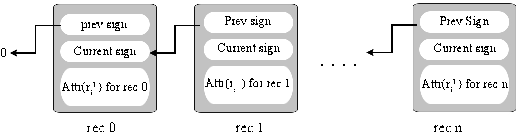
\includegraphics[width=\textwidth]{figs/blockchain.pdf}
			\caption{Idea of the Blockchain for the proposed system.}
			\label{fig:Blockchain}
		\end{figure}

	\section{Temporal Relational Databases} \label{sec:temporal database}
		 The main focus of this research is to build a trusted temporal relation using Blockchain technology that provides data provenance for the database system. In this section, we introduce the tools and concepts that were utilized in this research to establish a trusted temporal relation.
	%----------------------------------definition Temporal database----------------------------------
		\begin{defn}[Temporal database]
			Let $r$, be a relation in the database $D$. Denote the attributes of the relation as $attr(r)$. A temporal table of relation denoted $r^T$ is a table with attributes $attr(r^T) = attr(r_i) \cup \{timestamp, deleted\}$ where $timestamp$ is the time in which transactions on $r$ happened and $deleted$ is a flag showing whether or not that transaction was meant to delete a record from $r$. A temporal database denoted $D^T$ is the result of augmenting $D$ by $r^T$:

			\begin{center}
				{$D^T = D \cup \{{r^T}: r \in D \}$}
			\end{center}
		\label{dfn:temporal_database}
		\end {defn}

		The temporal database $D^T$ contains the entire history of the records ever existed in $D$.

		\begin{example}
			Given a normal relational table $r_1$ (Table \ref{table:normal_relational_table}) and a temporal table $r^T$ (Table \ref{table:temporal_table}), the $attr(r_1) = \{id, item, value\}$ and $attr(r^T)= \{id, item, value, updated, deleted\}$. The result of a few example queries are:

			\begin{itemize}
				\item {$q_1$: SELECT * FROM $r$ WHERE id = 22;}\\
				\textbf{Result:} $[(22,Pencil,7.50)]$
				\item {$q_2$: SELECT * FROM $r^T$ WHERE id = 22;}\\
				\textbf{Result:} $[(22,pencil,8.0,2018-03-21,False)$, \\$(22,pencil,7.50,2018-03-30,False)]$
				\item {$q_3$: SELECT * FROM $r$ WHERE id = 21;}\\
				\textbf{Result:} $[]$
				\item {$q_4$: SELECT * FROM $r^T$ WHERE id = 21;}\\
				\textbf{Result:} $[(21,ruler,3.25,2018-02-10,False)$, \\$(21,ruler,3.25,2018-02-20), True]$.
			\end{itemize}
			This example clearly shows that the temporal tables can provide data provenance for the records ever existed in the normal relations. For exmaple by having the temporal table ``$r^T$`` it could be seen that the record with ``$id = 22$`` used to have the value of ``$8.0$`` set in ``$2018-03-21$`` but then changed to ``$7.50$`` at ``$2018-03-30$``. Also, once there was a record with ``$id = 21$`` but deleted at ``$2018-02-20$`` and that is why the query $q_3$ does not return any results.
		\label{example:temporal_table}
		\end{example}

		\begin{center}
		\begin{table}[t]
			\centering
			\caption{Normal Relational Table $r_1$}
			\label{table:normal_relational_table}
			\begin{tabular}{p{4cm}p{4cm}p{4cm}}
				\hline
				id & item      & value  \\ \hline
				22 & Pencil    & 7.50 \\
				23 & Notebook & 12.0   \\ \hline
			\end{tabular}
		\end{table}

		\begin{table}[t]
			\centering
			\caption{Temporal Table $r^T$}
			\label{table:temporal_table}
			\begin{tabular}{p{1cm}p{2cm}p{3cm}p{3cm}p{2cm}}
				\hline
				id & item      & value  & timestamp  & deleted\\ \hline
				21 & Ruler    & 3.25\$  & 2018-02-10  &  False \\  
				21 & Ruler    & 3.25\$  & 2018-02-20  &  True \\
				22 & Pencil    & 8.0\$  & 2018-03-21  &  False \\
				22 & Pencil    & 7.50\$  & 2018-03-30  &  False\\
				23 & Notebook & 12.0\$  & 2018-04-01 & False \\ \hline
			\end{tabular}
		\end{table} 
		\end{center}

		The temporal database provides information about the timestamp in which the transactions on the database system occurred.
	%---------------------------------- End of Definition Temporal Database -----------------
	%---------------------------------- Defintion Time Domain -------------------------------
		\begin{defn}[Time domain]
			The time domain $\mathcal{T}$ consists of discrete timestamps $t_0,t_1,...,t_n$ in which transactions on tables $r \in D$ happened. The range of time domain is: $\mathcal{T} = [t_0,t_n]$ where the lower bound $t_0$ is the timestamp in which the first record added and the upper bound $t_n$ is the timestamp of the most recent transaction to the table $r$.
		\label{dfn:time_domain}
		\end{defn}

		\begin{example}
			The time domain of a temporal table $r^T$ (Table \ref{table:temporal_table}) is given by:
			$$\mathcal{T} = range(r^T[timestamp]) = [2018-02-10, 2018-04-01]$$
		\label{example:time_domain}
		\end{example}
	%---------------------------------- End of Definition Time Domain -----------------------
	%---------------------------------- Defintion Timestamps --------------------------------
		\begin{defn}[Timestamps]
			A timestamp $t_i \in \mathcal{T}$ is a particular position in the time domain, in which (a) particular transaction(s) happened. For example in the temporal table $r^T$ \ref{table:temporal_table}, ``2018-03-30'' is a timestamp in which the record with ``id = 22'' updated.
		\label{dfn:timestamp}
		\end{defn}
	%---------------------------------- End of Definition Timestamps ------------------------
	%---------------------------------- Defintion Timeline ----------------------------------
		\begin{defn}[Timeline]
			Let $u_1,u_2,...,u_n$ be the total number of transactions on the tables $r \in D$ at timestamps $t_j \in \mathcal{T}$, where $j=\{0,1,...,n\}$. These transactions could be represented as an ordered set points on a vector. This vector is called the {\textit timeline of transactions} for $r \in D$.
		\label{dfn:timeline}
		\end{defn}
		Figure \ref{fig:timeline} illustrates the concept of timeline.

		\begin{figure}
			\centering
			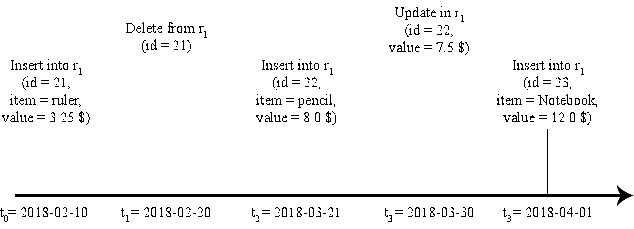
\includegraphics[width=\textwidth]{figs/timeline.pdf}
			\caption{Timeline.}
			\label{fig:timeline}
		\end{figure}

	Given a temporal database, for the sake of data analytics, it is a common practice to query for the form of a table in an specific timestamp. These queries could be answered by creating snapshot of the relation using the temporal table. 
	%---------------------------------- End of Definition Timeline --------------------------
	%---------------------------------- Defintion snapshot ----------------------------------
		\begin{defn}[Snapshot] 
			Given a temporal table $r^T \in D^T$ and a timestamp $t \in \mathcal{T}$, we denote $s(t)$ to be the table instance that obtained by calculating the $\{max(r^T[m])|t : m\in r)\}-r^T[deleted]$ for $\mathcal{T}\leq t$. A snapshot is a materialized version of $D(t) = \{s_1(t),s_2(t),...,s_n(t)\}$.
		\label{dfn:snapshot}
		\end{defn}

		\begin{example}
			Given a normal relational table $r_1$ (Table \ref{table:normal_table_2}), the temporal relational table $r^T$ (Table \ref{table:temporal_table_2}) contains the historical data of $r_1$. The snapshot of the $r_1$ at $t=2018-04-01$ could be generated as Table $\ref{table:normal_table_2_t}$.
		\label{example:snapshot_table}
		\end{example}

		\begin{center}
		\begin{table}
			\centering
			\small
			\caption{Normal Relational Table $r_1$}
			\label{table:normal_table_2}
			\begin{tabular}{p{4cm}p{4cm}p{4cm}}
				\hline
				id & item      & value  \\ \hline
				22 & Pencil    & 7.50 \\
				23 & Notebook & 12.0   \\ 
				24 & Console & 230.0 \\ \hline
			\end{tabular}
		\end{table}

		\begin{table}
			\centering
			\small
			\caption{Temporal Table $r^T$}
			\label {table:temporal_table_2}
			\begin{tabular}{p{1cm}p{2cm}p{3cm}p{3cm}p{2cm}}
				\hline
				id & item      & value  & timestamp  & deleted\\ \hline
				21 & Ruler    & 3.25  & 2018-02-10  &  False \\  
				22 & Pencil    & 8.0  & 2018-03-21  &  False \\
				22 & Pencil    & 9.0  & 2018-03-30  &  False\\
				23 & Notebook & 11.0  & 2018-04-01 & False \\
				22 & Pencil & 6.0  & 2018-04-01 & False \\
				21 & Ruler    & 3.25  & 2018-04-02  &  True \\
				23 & Notebook & 12.0  & 2018-04-02 & False \\ 
				22 & Pencil & 7.50  & 2018-04-05 & False \\ 
				24 & Console & 230.0  & 2018-04-05 & False \\ \hline
			\end{tabular}
		\end{table}
		\end{center}
		\begin{center}
		\begin{table}
			\centering
			\small
			\caption{Normal Relational Table $r_1$ at t = 2018-04-01}
			\label{table:normal_table_2_t}
			\begin{tabular}{p{4cm}p{4cm}p{4cm}}
				\hline
				id & item  & value  \\ \hline
				21 & Ruler & 3.25 \\
				22 & Pencil & 6.0   \\ 
				23 & Notebook & 11.0 \\ \hline
			\end{tabular}
		\end{table}
		\end{center}
	%---------------------------------- End of Definition snapshot --------------------------
	%---------------------------------- Begin of Blockchain  --------------------------------

	\section {Related Work} \label{sec:related_work}
		There has been a wide range of studies on ensuring the trustworthiness of records in a database from different perspectives. These studies range from establishing trust between nodes in a real-time distributed systems \cite{khayat2017trust} to secret sharing schemes in cloud databases \cite{dutta2013privacy} and utilizing logfiles for forensic purposes \cite{sinha2014continuous}. In this project, the assumption is that the preventive models are not able to stop the adversaries from manipulating the data of a relational database system, therefore a tamper-evident log table has been offered to evaluate whether or not the data has been altered. 

		Database audit logs contain valuable information such as any insertions, deletions, and modifications of the records performed in a database along with the timestamp of the performed tasks. The United States Department of Defense in its “Trusted Computer System Evaluation Criteria” document and under requirement 4 pointed out the importance of auditing the transactions in a computer system in a secure and efficient manner \cite{USDoD1985}. In this document also protecting the audit logs from modification or destruction has been stressed out.

		Analyzing audit logs for forensic purposes has been the topic of research by many scientists, however, since the trustworthiness of the results from log table analysis has a direct relationship with the authenticity of the records of the log file, a lot of studies have been carried out to make log tables tamper-proof. Haber {\it et al.}\cite{haber1991how} proposed a basic methodology by utilizing timestamping and hash chains in order to make unmodifiable historical records for digital documents. Peha in \cite{peha1999electronic} offered a method to detect log tampering by one way hashing and employing multiple trusted notaries to keep track of all transactions. The author argued that if any notary decided to falsify the transaction, the attempt is discovered by other notaries. Snodgrass {\it et al.} \cite{snodgrass2004Tamper} also offered one-way hashing mechanism and employed trusted notaries, however in order to enhance the security of the method offered by Peha, they offered to hash the records with a timestamp of previous transaction modification. Schneier {\it et al.}\cite{schneier1998cryptoraphic} offered a cryptographic-based mechanism to create hash chains and make the log files nearly impossible for the attacker to alter. The validity of the transactions was also done by trusted third-parties who have the cryptographic keys.

		However the aforementioned researches might have promising results to protect the historical records from being compromised by an outsider, but they have one thing in common which is the role of an insider to carry out malicious attacks is forgotten. Also hiring third-party software/hardware may bring up a lot of privacy concerns. Therefore, unlike the mentioned works, not only our proposed system does not require a third-party notary to attest the authenticity but also it does not put trust on any user of the system.

		The role of privileged users in acting maliciously in a database has been discussed by many researchers \cite{crosby2009tamper-evident} \cite{wagner2018detect}. Liu {\it et al.} offered a network-based auditing mechanism which also keeps track of privileged users' activity and performs audit analysis through event correlation. Wagner {\it et al.} \cite{wanger2017carving} proposed a mechanism to detect database file tampering by looking for inconsistencies in the database's storage. The authors argued that the databases follow patterns in storage which even the privileged users have no access to. Therefore, if a record is deleted maliciously in the log file, the inconsistency in the storage is evident for a period of time. Unlike mentioned proposed methods, our system uses inherent to RDBMS tools and does not require a network-level-auditing mechanism or having access to the server's storages, therefore it could be easily implemented on remote servers and relational databases on cloud storages. Also, our proposed system not only discovers maliciously deletion of the records but also identifies any malicious modification without any time constraints.

		For the sake of gathering verifiable pieces of evidence, in our proposed system, any changes to the database regardless of the users' access privileges need to be tracked. This action could be done by utilizing inherent to DBMS tools. Fabbri {\it et al.} \cite{fabbri2013select} extensively talked about SELECT triggers which are inherent RDBMS functions, required database specifications and efficient implementation techniques for data auditing. Hauger {\it et al.}\cite{hauger2014information} also discussed the use of triggers in the database for forensic purposes. Triggers are supported by RDBMS which makes them a good candidate to be used in our proposed system however, it is naive to assume that a simple trigger solely is secure enough to be used for forensic purposes. Therefore we propose to use the Blockchain technology to make immutable chains of transactions that are captured by database triggers.

		The first attempt to use chained hashes for securing data from tampering is known to be done by Haber {\it et al.} \cite{haber1991how} where the authors proposed a methodology to securely timestamp the digital files and create digital signatures and hash chains. This work was then improved by Schneier {\it et al.} \cite{schneier1998cryptoraphic} \cite{schneier1999minimizing} \cite{schneier1999secure} by offering to exchange secret codes with a trusted third party who is able to verify the authenticity of the chain. They offered a method to change the shared secret as the new transaction occurs, therefore since the attackers do not have the previous secret codes, it is impossible for them to alter any records which were previously added. Our proposed method is similar to the mentioned works in this aspect that our historical records are chained together using the digital signatures, however, we use asymmetric encryption to generate digital signatures that removes the need of the third-parties to attest the authenticity of the transactions. The asymmetric encryption method also enables anybody to verify signatures without revealing the users' secrets.